%---------------------------------------------------
% Nombre: capitulo2.tex  
% 
% Texto del cap�tulo 2
%---------------------------------------------------

\chapter{Preprocesado}
\label{preprocesado}

En este cap�tulo enunciaremos el proceso de preprocesado llevado a cabo durante la realizaci�n de la pr�ctica. Cabe destacar, que por facilitar la comprensi�n todo el proceso se enuncia en este cap�tulo, pero hay ciertos puntos como el del proceso de undersampling (secci�n \ref{undersampling}) y el de corte de las im�genes  (secci�n \ref{cut}) que surgen fruto de cambios e ideas en el proceso de aprendizaje y entrenamiento de las redes neuronales. 

\section{Resize data}

Como veremos en el cap�tulo de conclusi�n, uno de los requisitos y mayores problemas que esta pr�ctica a ofrecido han sido las limitaciones de memoria tanto de principal para computo como de memoria secundaria para almacenar todas las im�genes y sus diferentes versiones. Con el fin de poder manejar estas m�s eficientemente se ha realizado un resize de las mismas a tama�o de 256x256px, para ello hemos seguido el siguiente script en R. 

\lstset{language=R, breaklines=true, basicstyle=\footnotesize}
\lstset{numbers=left, numberstyle=\tiny, stepnumber=1, numbersep=-2pt}
\begin{lstlisting}
  #-------------------------------------------------------------------------------

  # Clear workspace
  rm(list=ls())

  #-------------------------------------------------------------------------------
  # Load and pre-process images
  #-------------------------------------------------------------------------------

  # Set run parameters parameters
  test_img_path <- "."
  width  <- 256
  height <- 256


  #-------------------------------------------------------------------------------
  # Load and pre-process train images
  #-------------------------------------------------------------------------------

  # Load EBImage library
  library(EBImage)

  # Load images into a dataframe
  library(gsubfn)
  img_file_list <- list.files(path = test_img_path, pattern = "*.jpg", full.names = TRUE, recursive = TRUE)

  train_df <- data.frame()

  for(i in 1:length(img_file_list)) {
    img_file_name <- img_file_list[i]
    #img_class <- strapplyc(img_file_list[i], ".*/Type_(.*)/")[[1]]
    img <- readImage(img_file_name)
    img_resized <- resize(img, w=width, h=height)
    
    name <- paste("reducidas",img_file_name, sep="/")
    dir.create("reducidas", showWarnings = FALSE)
    writeImage(img_resized, name)
    
  }  
\end{lstlisting}

Con este simple script podemos preprocesar las im�genes originales y reducir�as de tama�o de manera que son mas f�cilmente manejables, pero esto nos da un problema asociado y es que estamos modificando los datos originales.


\begin{figure}[H]
	\centering
		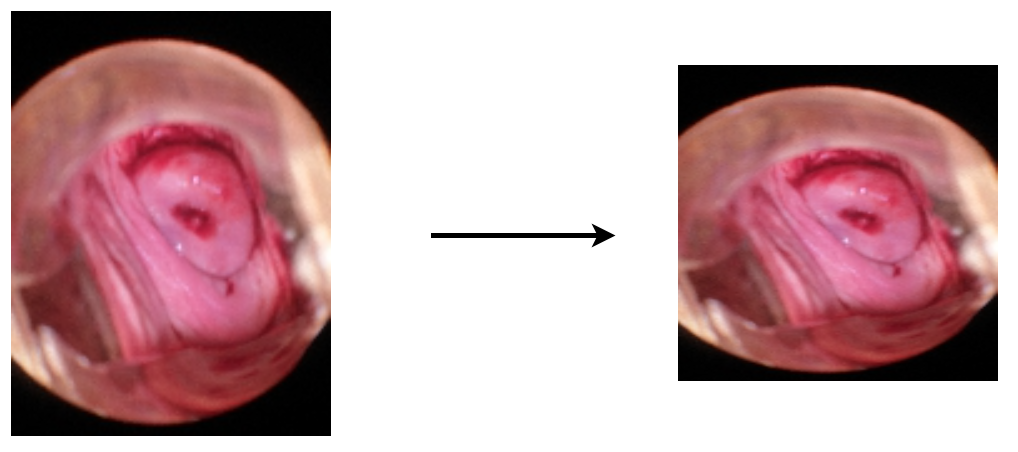
\includegraphics[scale=0.4]{./Capitulo2/imagenes/resize.png}
		\caption{Deformaci�n de la imagen al redimensionar.}
	\label{resize}
\end{figure} 

Tal y como podemos apreciar en la figura \ref{resize} si una imagen rectangular la `obligamos' a ser cuadrada, estamos deformando el contenido por lo que ya tendremos otra imagen distinta de la original,  a este problema la estudiaremos en la siguiente secci�n. 

\section{Cut data}
\label{cut}

Siguiendo con el ejemplo de la secci�n anterior, la soluci�n a la deformaci�n de la imagen pasa por cortar al ratio de aspecto 1:1 y posteriormente redimensionar para tener im�genes de menos peso. Este paso, puede explicarse con la imagen \ref{crop}.

\begin{figure}[H]
	\centering
		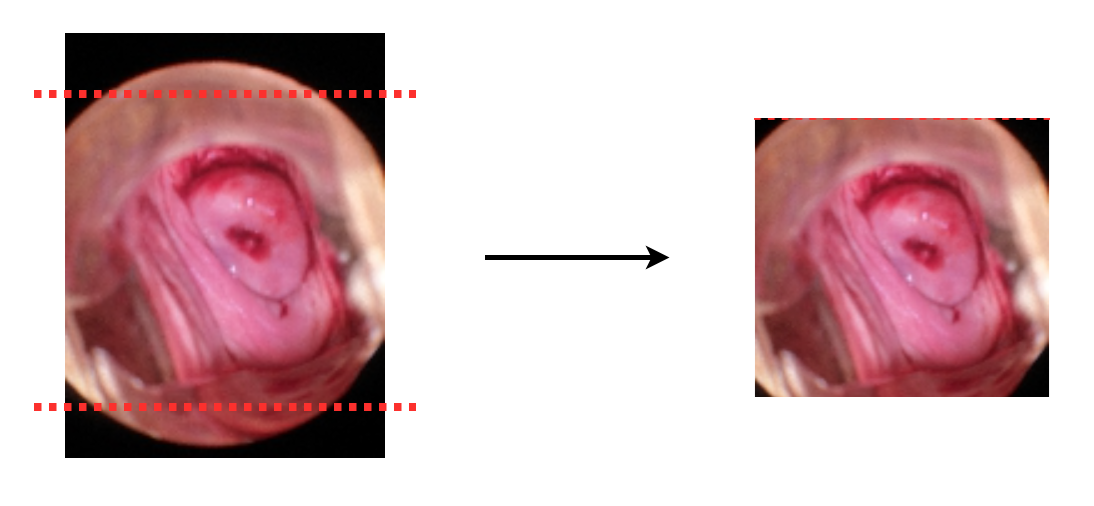
\includegraphics[scale=0.4]{./Capitulo2/imagenes/crop.png}
		\caption{Cortado de la imagen.}
	\label{crop}
\end{figure} 

La altura de la imagen debe ser por tanto igual al ancho de la misma y para ello, debemos quitar los espacios que vemos en la imagen anterior, tras lo cual tendremos una imagen cuadrada pero sin deformar el contenido, adem�s de quitar partes de la imagen que en m�s del 90\% de los casos no tienen importancia. Para calcular el corte hemos usado la ecuaci�n \ref{eq:corte}, que nos da el valor que deberemos substraer de la imagen original tanto por la parte superior como por la inferior. 

\begin{equation} 
corte=\frac{height-widht}{2}
\label{eq:corte}
\end{equation}

El script que usamos para este objetivo es el siguiente:

\lstset{language=R, breaklines=true, basicstyle=\footnotesize}
\lstset{numbers=left, numberstyle=\tiny, stepnumber=1, numbersep=-2pt}
\begin{lstlisting}
  #-------------------------------------------------------------------------------
  # This script cut the images to prevent original data deformation 
  #-------------------------------------------------------------------------------


  #setwd("D:/Facultad/Master/Segundo cuatrimestre/SIGE/PracticaFinal")
  # Clear workspace
  rm(list=ls())

  # Set run parameters parameters
  test_img_path <- "."

  # Load EBImage library
  library(EBImage)
  # Load images into a dataframe
  library(gsubfn)
  img_file_list <- list.files(path = test_img_path, pattern = "*.jpg", full.names = TRUE, recursive = FALSE)
  
  img_file_list
  dir.create("crop", showWarnings = FALSE)
  for(i in 1:length(img_file_list)) {
    
    img_file_name <- img_file_list[i]
    name <- paste("crop",img_file_name, sep="/")
    print(name)
    if(!file.exists(name)){
      img <- readImage(img_file_name)
      width <- dim(img)[1]
      heigth <- dim(img)[2]
      if (width < heigth){ 
        cut <- (heigth-width)/2
        p <- heigth-cut
        img2 <- img[0:width,cut:p,]
      }else{
        cut <- (width-heigth)/2
        p <- width-cut
        img2 <- img[cut:p,0:heigth,]
      }

      writeImage(img2, name)
    }
    
  }
  print("Finalizado")
\end{lstlisting}

\section{Data Aumentation}
\label{aumentation}
Uno de los principales problemas en \textit{deep learning} es la falta de datos. Para ello, pueden usarse t�cnicas de \textit{data aumentation} que consisten en aplicar ligeras transformaciones a las im�genes para conseguir un conjunto de entrenamiento mayor. Para ello, hemos usado dos vertientes, una con R (siguiente script) con la que obtenemos im�genes modificadas en ficheros separados para poder ir combin�ndolas como deseemos, y por �ltimo, en el c�digo Python que veremos en puntos siguientes, sobre estas volv�amos a aplicar una serie de cambios aumentando por tanto el data set bastante.   

\lstset{language=R, breaklines=true, basicstyle=\footnotesize}
\lstset{numbers=left, numberstyle=\tiny, stepnumber=1, numbersep=-2pt}
\begin{lstlisting}

  #-------------------------------------------------------------------------------

  # Clear workspace
  rm(list=ls())

  #-------------------------------------------------------------------------------
  # Load and pre-process images
  #-------------------------------------------------------------------------------

  # Set run parameters parameters
  train_img_1_path <- "./Type_1"
  train_img_2_path <- "./Type_2"
  train_img_3_path <- "./Type_3"


  #-------------------------------------------------------------------------------
  # Load and pre-process train images
  #-------------------------------------------------------------------------------

  # Load EBImage library
  library(EBImage)

  # Load images into a dataframe
  library(gsubfn)
  img_file_1_list <- list.files(path = train_img_1_path, pattern = "*.jpg", full.names = TRUE, recursive = TRUE)
  img_file_2_list <- list.files(path = train_img_2_path, pattern = "*.jpg", full.names = TRUE, recursive = TRUE)
  img_file_3_list <- list.files(path = train_img_3_path, pattern = "*.jpg", full.names = TRUE, recursive = TRUE)


  #train_df <- data.frame()

  #Hacemos 3 bucles porque tienen tama?os distintos cada clase.

  Imagenes<-function(image,type) {
    img_file_name <- image
    
    img <- readImage(img_file_name)
    
    if(type=="flip"){
      img <- flip(img)
    }
    
    if(type=="flop"){
      img <- flop(img)
    }
    
    if(type=="rot"){
      img = rotate(img, 90, bg.col = "white")
    }
    if(type=="trans"){
      img_t = transpose(img)
    }
    
    #print("IMG_FILE_NAME")
    #print(img_file_name)
    
    salida <- substr(img_file_name, 0, 8)
    name <- paste(salida,type, sep="/")
    salida <- substr(img_file_name, 10,nchar(img_file_name) )
    #print("salida")
    #print(salida)
    salida <- paste(type,salida, sep="-")
    
    name2 <- paste(name,salida, sep="/")
    #print("NAME2")
    #print(name2)
    
    dir.create(name, showWarnings = FALSE)
    writeImage(img, name2)
  }



  tipos<-function(imagen){
    Imagenes(imagen,"flip")
    Imagenes(imagen,"flop")
    Imagenes(imagen,"rot")
    Imagenes(imagen,"trans")
  }

  for(i in 1:length(img_file_1_list)) {
    tipos(img_file_1_list[i])
  }


  for(i in 1:length(img_file_2_list)) {
    tipos(img_file_2_list[i])
  }

  for(i in 1:length(img_file_3_list)) {
    
    tipos(img_file_3_list[i])
    
  }

  print("FINALIZADO")

        
\end{lstlisting}

\section{Undersampling}
\label{undersampling}

Por �ltimo, en nuestro proceso de pre-procesado, descubrimos que las clases mostraban cierto desequilibrio. Concretamente, la clase1 frente a clase 3 de 1,66, y de clase 1 frente a clase 2 de 2,35. Aunque no es mucho, est�n por encima del 1,5, valor a partir del cual se considera un problema de clase desequilibradas. 

Para intentar solventar este problema, quitamos algunas im�genes de las clases mayoritarias intentando siempre que las im�genes originales estuvieran presentes entre las seleccionadas, de manera que se suprimieron algunas de las transformaciones obteniendo ratios de balanceo por debajo del 1.5. Esta soluci�n, al evaluar en test, lejos de mejorar empeoraba el modelo ya que como hemos visto en \ref{aumentation} el principal problema a solventar en esta competici�n es la falta de informaci�n en training y con esta t�cnica, aunque igualamos clases, perdemos informaci�n que puede ser decisiva. 

\pagebreak
\clearpage
%---------------------------------------------------